\documentclass{beamer}[10]
\usepackage{beamerthemesplit}
\usepackage{hyperref}
\usepackage{amsmath}
\usepackage{graphicx}
\usepackage{caption}
\usepackage{listings}

%New commands
\newcommand{\clash}{C$\lambda$aSH}
\newcommand{\ve}[1]{\mathbf{\textcolor{blue}{#1}}}
\newcommand{\horspace}{\hspace{15pt}}
\providecommand{\e}[1]{\ensuremath{\times 10^{#1}}}
\newcommand{\matlab}{MATLAB}
\newcommand{\mytilde}{{\raise.17ex\hbox{$\scriptstyle\sim$}}}

%Colours
\definecolor{custom_blue}{RGB}{74,140,188}


%Set up the slides
\mode<presentation>
\captionsetup{font=scriptsize,labelfont=scriptsize}
\usetheme[numbers,totalnumber,compress,sidebarshades]{PaloAlto}
\setbeamertemplate{footline}[frame number]
\usecolortheme[named=custom_blue]{structure}
\useinnertheme{circles}
\usefonttheme[onlymath]{serif}
\setbeamercovered{transparent}
\setbeamertemplate{blocks}[rounded][shadow=true]
\logo{\includegraphics[width=2cm]{figs/icon_dark.pdf}}

%Define the sidebar
\makeatletter
\setbeamertemplate{sidebar \beamer@sidebarside}
{
	\beamer@tempdim=\beamer@sidebarwidth
	\advance\beamer@tempdim by -6pt
	\vspace{10 pt}
	\insertverticalnavigation{\beamer@sidebarwidth}
	\vfill
	\ifx\beamer@sidebarside\beamer@lefttext%
	\else
	\usebeamercolor{normal text}
	\llap{\usebeamertemplate***{navigation symbols}\hskip0.1cm}
	\vskip2pt
	\fi
}

%Default style for listings
\lstdefinestyle{haskellStyle}{
	xleftmargin=5pt,
	language=Haskell,
	numbers=left,
	stepnumber=1,
	numbersep=5pt,
	tabsize=4,
	showspaces=false,
	showstringspaces=false,
	basicstyle=\scriptsize,
	columns=flexible
}
\lstset{style=haskellStyle}

\title{Numerical mathematics on FPGAs using \clash{}}
\subtitle{From Haskell to a hardware accelerator}
\author{Martijn Bakker}
\institute{Computer Architecture for Embedded Systems (CAES) \\ University of Twente}
\date{\today{}}

\begin{document}

\begin{frame}
\titlepage
\end{frame} 

\begin{frame}
\frametitle{Overview}
\tableofcontents
\end{frame} 

\section{Functional programming}

\begin{frame}
	\frametitle{Properties}

	\begin{itemize}
	\item Main building block: functions
	\vspace{15pt}
	\item No assignments, only \emph{unchangeable} definitions
	\item No statements, only expressions
	\item `Variables` that cannot vary
	\vspace{15pt}
	\item The execution of a program is a function evaluation
	\end{itemize}
\end{frame}

\begin{frame}
	\frametitle{Resulting features}
	
	\begin{itemize}
		\item No global, mutable state
		\item No side effects
		\item Pure functions
	\end{itemize}
	\begin{itemize}
		\item Lazy evaluation
		\item Higher-order functions
		\item Strong type system
		\item Partial function application
		\item Function composition
		
		\vspace{15pt}
		\item Clear structure of the program, similar to mathematics
	\end{itemize}
\end{frame}


\begin{frame}[fragile]
	\frametitle{Example of functional programming}
	\lstinputlisting[caption=A very short introduction to functional programming, language=Haskell]{material/fpdemo.hs}
\end{frame}	
	

\section{FPGA}
\begin{frame}
	\frametitle{The Field-Programmable Gate Array}
	\begin{itemize}
		\item 'Programmable hardware'
		\item Create your own circuit instead of a list of instructions
	\end{itemize}
	
	\begin{figure}
		\centering
		\includegraphics[width=\columnwidth]{figs/fpga.jpg}
		\caption{FPGA structure}
	\end{figure}
\end{frame}

\begin{frame}
	\frametitle{Why would you want to use an FPGA?}
	Advantages over CPUs
	\begin{itemize}
		\item High throughput
		\item Low \emph{guaranteed} latency
		\item Low power use
		\item Support for new "instructions"
	\end{itemize}
	\vspace{15pt}
	Advantages over ASICs
	\begin{itemize}
		\item Reconfigurability 
	\end{itemize}
\end{frame}

\begin{frame}
	\frametitle{Drawbacks}
	\lstinputlisting[caption=A single AND-gate\, specified in VHDL, language=VHDL]{material/andgate.vhdl}
\end{frame}

\begin{frame}
	\frametitle{Drawbacks}
	
	\begin{enumerate} 
	\item FPGA development is \textbf{hard}
	
	\begin{itemize}
		\item Vendor-specific, closed-source tools
		\item Small communities
		\item Ancient HDLs
		\item Synthesis, debugging and verification is a slow process
	\end{itemize}
	
	\vspace{15pt}
	\item FPGAs cannot be reconfigured as quickly as CPUs
	
	\vspace{15pt}
	\item FPGAs run at lower clock speeds than ASICs
	\end{enumerate}
\end{frame}


\section{\clash{}}
\begin{frame}
	\frametitle{\clash{} - What?}
	\begin{itemize}
		\item CAES Language for Synchronous Hardware 
		\vspace{15pt}
		\item A library for the specification of hardware in Haskell. 
		\item Includes a compiler: generation of VHDL and Verilog
		\item Written by Christiaan Baaij at CAES
		\vspace{15pt}
		\item \href{http://www.clash-lang.org/}{www.clash-lang.org}
		\end{itemize}
\end{frame}

\begin{frame}
	\frametitle{\clash{} - Why?}
	Similarities between hardware and functional programming
	\begin{itemize}
		\item Hardware consists of largely combinatorial parts: pure functions
		\item Combinatorial circuits contain a dependency tree: function dependencies
		\item Higher-order functions
	\end{itemize}
\end{frame}

\begin{frame}
	\frametitle{\clash{} - Apparent issues?}
	\begin{itemize}
		\item Hardware has a mutable state
		\item Functional programming has no mutable states
	\end{itemize}
	
	\pause
	\vspace{15pt}
	Solution: the Mealy machine.
\end{frame}

\begin{frame}
	\frametitle{The Mealy machine}
	\begin{figure}
		\centering
		\includegraphics[width=1\columnwidth]{figs/mealy_machine.png}
		\caption{Block diagram describing a Mealy machine. The loop gets executed once every clock cycle.}
	\end{figure}
\end{frame}
	
\begin{frame}
	\frametitle{Example}
	\lstinputlisting[caption=A basic multiply-accumulate circuit specification in \clash{}]{material/clashexample.hs}
\end{frame}


\begin{frame}
	\frametitle{Wrap-up of introduction}
	\begin{figure}
		\centering
		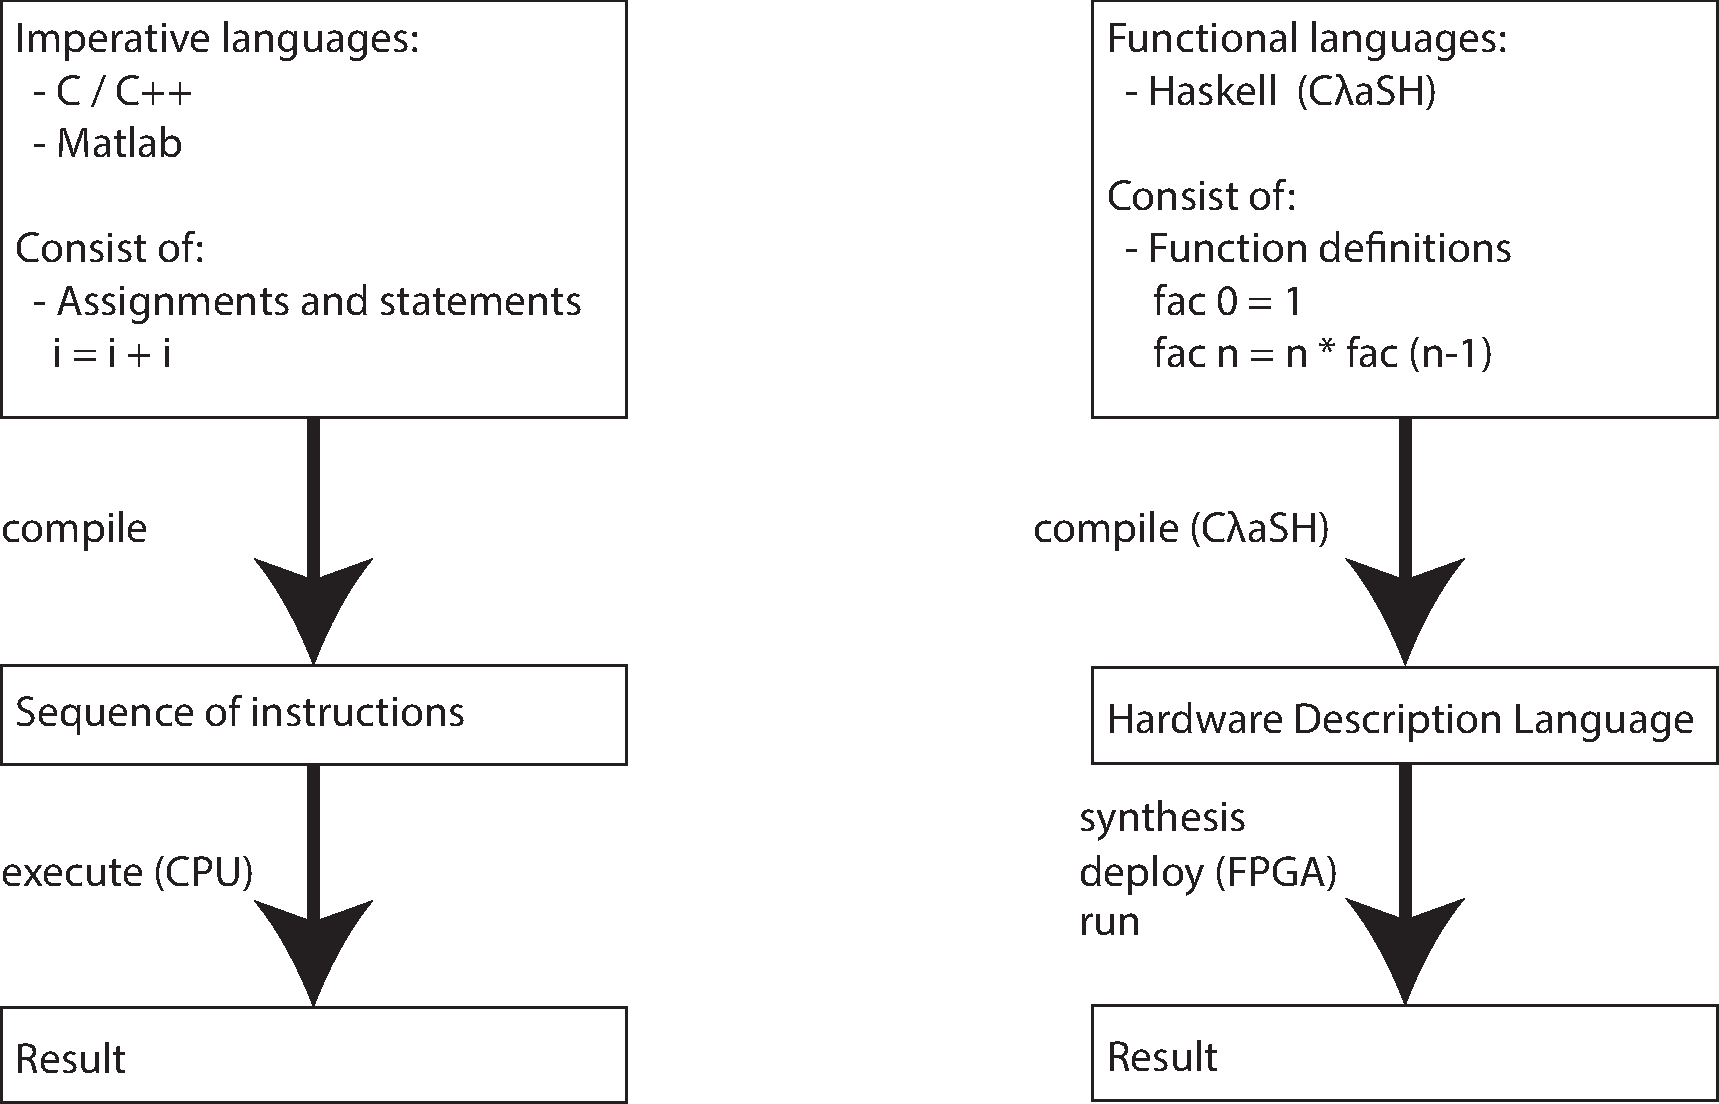
\includegraphics[width=\columnwidth]{figs/functional-vs-imperative}
	\end{figure}
\end{frame}

\section{Problem definition and breakdown}
\begin{frame}
	\frametitle{Definition}
	
	The \textbf{feasibility} and \textbf{performance} of performing \textbf{numerical approximations} to \textbf{ODEs} on an FPGA with hardware specified in \clash{}.
	
	\begin{enumerate}
		\item \textbf{Feasibility}: does the most simple version work?
		\item \textbf{Performance}: comparison with a desktop CPU
		\item \textbf{Numerical approximations}: simple integration schemes (Euler, RK2, RK4)
		\item \textbf{ODEs}: 4 coupled first order differential equations with constant coefficients (4x4 matrix)
		\item \textbf{FPGA}: a Terasic SoCKit development board, containing an Altera Cyclone V SoC FPGA
	\end{enumerate}
\end{frame}

\begin{frame}
	\frametitle{Breakdown - requirements for the system}
	
	\begin{itemize}
		\item Number representation
		\item Number storage
		\item Control protocol
		\item Supplying a suitable clock frequency	
	\end{itemize}
		
	\begin{enumerate}
		\item Programming
		\item Getting matrix constants and initial values in
		\item Controlling and monitoring the state
		\item Performing the actual computation
		\item Getting results out of the FPGA (go to 3)
	\end{enumerate}
	
\end{frame}

\begin{frame}
	\frametitle{Number representation}
	
	\begin{itemize}
		\item Floating point or fixed point?
		
		\pause
		\vspace{15pt}
		\item \clash{} only supports fixed point
		
		\pause
		\vspace{15pt}
		\item Signed fixed point with 8 integer bits and 24 fractional bits
		\item Total width: 32 bits
		\item Integer range: [-128 .. 127]
		\item ULP\footnote{Unit of least precision}: $2^{-24} \approx 6\e{-8}$, roughly 7 decimal digits.
	\end{itemize}
	
\end{frame}

\begin{frame}
	\frametitle{Number storage}
	
	\begin{itemize}
		\item Registers\footnote{Direcly accessible on-chip: latches}, SRAM\footnote{Static RAM, on-chip, single cycle access delays} or SDRAM\footnote{Synchronous Dynamic RAM, off-chip, 'high' latency}?
		\pause
		\vspace{15pt}
		\item All variables get updated every single cycle.
		\item All data fits in the registers.
		\item No need for SRAM or SDRAM.
	\end{itemize}
	
\end{frame}

\begin{frame}
	\frametitle{Supplying a suitable clock frequency}
	
	\begin{itemize}
		\item A higher* clock frequency means higher throughput 
		\pause
		\vspace{15pt}
		\item *up to a certain limit, otherwise your system fails.
		\item Output stabilization of the combinatorial circuits takes time.
		\pause
		\vspace{15pt}
		\item FPGA contains a crystal (50 MHz) and PLL\footnote{Phase-Locked Loop} circuits.
		\item \clash{} + IO + Altera PLL = non-deterministic behaviour.
		\item Solution: a simple integer frequency divider.
	\end{itemize}
\end{frame}

\section{\clash{} project overview}

\begin{frame}
	\frametitle{Actual computation - External Types}
	\lstinputlisting[caption=\clash{} topEntity for the ODE solver, firstline=14]{material/comp_types.hs}
\end{frame}

\begin{frame}
	\frametitle{Actual computation - Internal Types}
	\lstinputlisting[caption=Internal types for the ODE solver, firstline=1, lastline=11]{material/comp_types.hs}
\end{frame}

\begin{frame}
	\frametitle{Actual computation - Equation}
	\begin{equation}
		\ve{x}' = \begin{bmatrix}
		c_{1} & c_{2} \\ c_{3} & c_{4} \\
		\end{bmatrix} \ve{x}
	\end{equation}
	\lstinputlisting[caption=Computing the derivative]{material/comp_eq.hs}
\end{frame}

\begin{frame}
	\frametitle{Actual computation - Scheme}
	\begin{equation}
		\ve{x}_{k+1} = 
		\begin{cases} 
			\ve{x}_{k} + h\ve{x}_{k}' 		& \text{if } t_{k} < t_{max} \\
			\ve{x}_{k} 						& \text{otherwise} 
		\end{cases} 
	\end{equation}
	\lstinputlisting[caption=Eulers method]{material/comp_scheme.hs}
\end{frame}

\begin{frame}
	\frametitle{Actual computation - Control}
	\lstinputlisting[caption=Controlling the ODE solver (important lines start with '!'),basicstyle=\tiny]{material/comp_control.hs}
\end{frame}


\begin{frame}
	\frametitle{An overview of the entire system}
	\begin{figure}
		\centering
		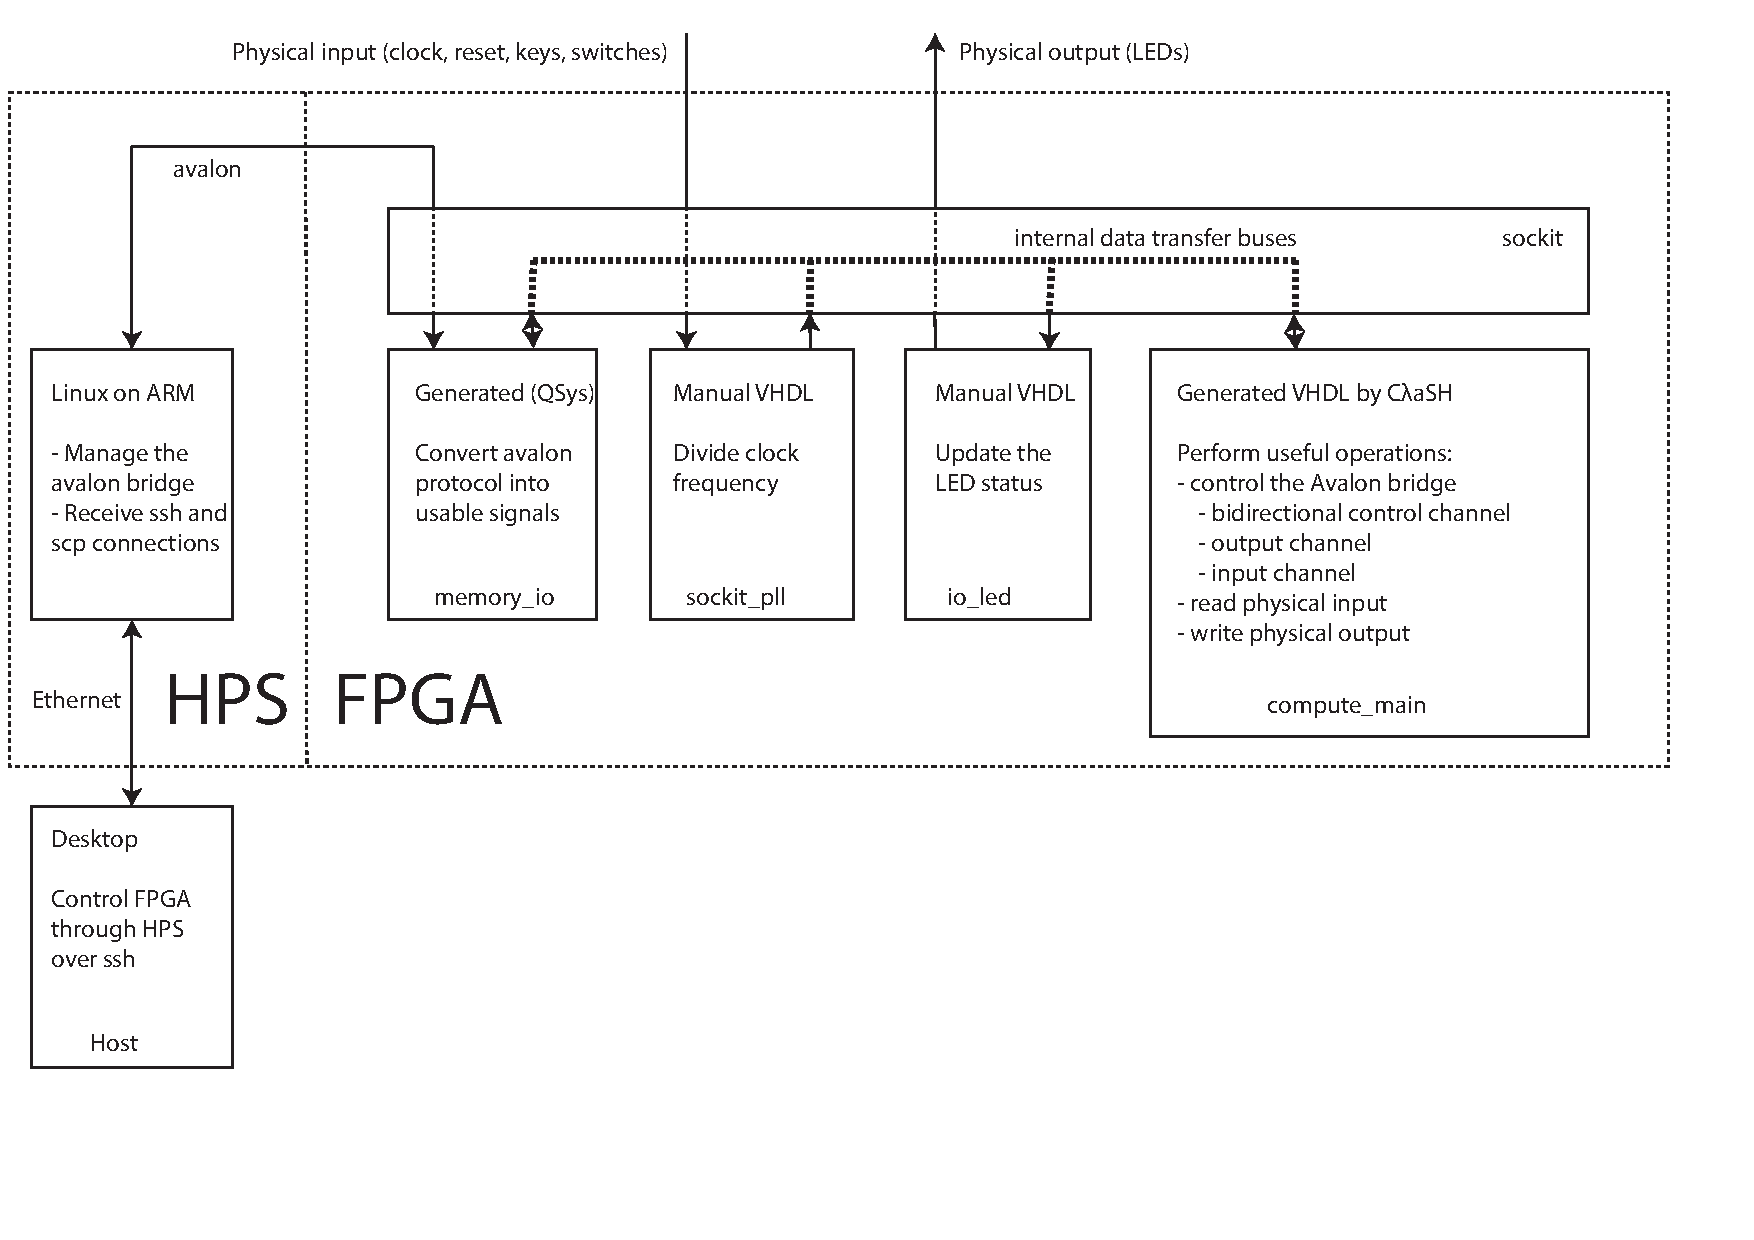
\includegraphics[width=\columnwidth]{figs/diagram}
	\end{figure}
\end{frame}

\section{Results}
\begin{frame}
	\frametitle{Results}
	\begin{itemize}
		\item Each solution plot contains 3 curves
		\begin{enumerate}
			\item FPGA-approximation
			\item \matlab{}-approximation (same functionality as FPGA)
			\item Analytical or obtained from ode45(), the real solution
		\end{enumerate}
		\item Each error plot contains at least 2 curves
		\begin{enumerate}
			\item FPGA - real
			\item FPGA - \matlab{} approximation
		\end{enumerate}
		\vspace{15pt}
		\pause
		\item \matlab{} uses IEEE 754 double precision floating point
		\item FPGA uses 8/24 signed fixed point. 
	\end{itemize}
\end{frame}

\begin{frame}
	\frametitle{Simple oscillation - I \horspace{} $x(t) = 50 \cos(t)$}
	\begin{figure}
		\centering
		\includegraphics[width=\columnwidth]{figs/euler_o1_ts=0,01_os=1}
		\label{f:euler_o1_ts=0,01_os=1}
		\caption{The final error is $\approx 30$ (h = 0.01)}
	\end{figure}
\end{frame}

\begin{frame}
	\frametitle{Simple oscillation - II \horspace{} $x(t) = 50 \cos(t)$}
	\begin{figure}
		\centering
		\includegraphics[width=\columnwidth]{figs/euler_o1_ts=0,0001_os=100}
		\label{f:euler_o1_ts=0,0001_os=100}
		\caption{The final error decreased by a factor 150 (h = 1\e{-4})}
	\end{figure}
\end{frame}

\begin{frame}
	\frametitle{Simple oscillation - III \horspace{} $x(t) = 50 \cos(t)$}
	\begin{figure}
		\centering
		\includegraphics[width=\columnwidth]{figs/euler_o1_ts=0,0000001_os=1000}
		\label{f:euler_o1_ts=0,0000001_os=1000}
		\caption{Breakdown of the number representation (h = 1\e{-7})}
	\end{figure}
\end{frame}

%\begin{figure}
%\begin{align}
%\ve{x}'_k 	 &= f(t_{k},\ve{x}_{k})  \\ 
%\ve{s}_{k,1} &= f(t_{k},\ve{x}_{k}) \\
%\ve{s}_{k,2} &= f(t_{k} + h, \ve{x}_{k} + h\ve{s}_{k,1}) \\
%\ve{x}_{k+1} &=	\begin{cases} 
%\ve{x}_{k} + h \frac{\ve{s}_{k,1} + \ve{s}_{k,2}}{2} 		& \text{if } t_{k} < t_{max} \\
%\ve{x}_{k} 													& \text{otherwise} 
%\end{cases} 
%\end{align}
%\caption{Runge-Kutta, second order}
%\end{figure}


\begin{frame}
	\frametitle{Switching equations}
	
	\begin{itemize}
		\item Eulers method (first order) to RK2 (second order)
		\item Simple oscillations to 4 coupled equations
		\item Matrix chosen such that all eigenvalues negative
	\end{itemize}

	\begin{equation}
	\ve{x}' = \begin{bmatrix} 
	2 & 3 & 2 & 0 \\
	-5 & -5 & -3 & 1 \\
	3 & -1 & -2 & -3 \\
	4 & 2 & 2 & -3 \\
	\end{bmatrix} \ve{x} 
	\hspace{20pt} \text{with} \hspace{20pt} 
	\ve{x}(t_{0}) =\begin{bmatrix} 7 \\ 5 \\ 7 \\ 5 \end{bmatrix} 
	\end{equation}
	
\end{frame}

\begin{frame}
	\frametitle{RK2 - I}
	\begin{figure}
		\centering
		\includegraphics[width=\columnwidth]{figs/rk2_ts=0,01_os=1}
		\label{f:rk2_ts=0,01_os=1}
		\caption{A high value of h, maximum error $\approx 0.3$ (h = 0.01)}
	\end{figure}
\end{frame}

\begin{frame}
	\frametitle{RK2 - II}
	\begin{figure}
		\centering
		\includegraphics[width=\columnwidth]{figs/rk2_ts=0,0000005_os=1000}
		\label{f:rk2_ts=0,0000005_os=1000}
		\caption{A very low value of h, maximum error $\approx 0.2$ (h = 5\e{-7})}
	\end{figure}
\end{frame}

\begin{frame}
	\frametitle{RK4}
	\begin{figure}
		\centering
		\includegraphics[width=\columnwidth]{figs/rk4_ts=0,00001_os=100}
		\label{f:rk4_ts=0,00001_os=100}
		\caption{For all tested values of h, (h = 1\e{-5})}
	\end{figure}
\end{frame}

\begin{frame}
	\frametitle{Euler revisited}
	\begin{figure}
		\centering
		\includegraphics[width=\columnwidth]{figs/euler_rv_ts=0,0001_os=10}
		\caption{Euler outperforming both RK2 and RK4, (h = 1\e{-4})}
		\label{f:euler_rv_ts=0,0001_os=10}
	\end{figure}
\end{frame}

\section{Performance}
\begin{frame}
	\frametitle{Results}
	\tiny
	\begin{table}
	\caption{\scriptsize Eulers method, sorted by iterations per second.}
	\label{t:performance}
	\begin{tabular}{l l l l l l}
		\textbf{Device} & \textbf{Iterations} & \textbf{time (s)}	& \textbf{Output interrupts}	& \textbf{Iterations per second (\e{6})} \\  
		CPU - C++ - int		& 1\e{8} 	& 1,35		& 1			& 74,1 	\\
		FPGA 				& 1\e{8} 	& 2,18		& 1			& 45,8 	\\
		FPGA 				& 1\e{8} 	& 2,25		& 1\e{3}	& 44,4 	\\
		FPGA 				& 1\e{8} 	& 2,30		& 1\e{4}	& 43,4 	\\
		FPGA 				& 1\e{8} 	& 3,27		& 1\e{5}	& 30,6 	\\
		FPGA 				& 1\e{7} 	& 0,39		& 1			& 25,6 	\\
		FPGA 				& 1\e{6} 	& 0,21		& 1			& 4,76 	\\
		CPU - C++ - float	& 5\e{7} 	& 58,1		& 1			& 0,86 	\\
		FPGA 				& 1\e{5} 	& 0,19		& 1			& 0,53 	\\
		CPU - Haskell - float& 1\e{6}	& 3,23		& 1			& 0,31	\\		
		CPU - \matlab{}	- float	& 1\e{7}& 304		& 1			& 0,03	\\
	\end{tabular}
	\end{table}
\end{frame}

\begin{frame}
	\frametitle{Notes}
	\begin{itemize}
		\item FPGA for "low-power, cost-sensitive design needs"
		\item No automatic derivation of the optimal clock frequency
		\item 4x4 matrix equation only used \mytilde{}10\% of the FPGA space
		\item Power usage is \mytilde{} 2 orders of magnitude lower than the CPU
		\item CPUs are heavily optimized for fast integer arithmetic
	\end{itemize}
\end{frame}

\section{Demo}
\begin{frame}
	\frametitle{The entire process takes \mytilde{}10 minutes}
	\begin{enumerate}
		\item \clash{} - Windows/Linux
		\item Synthesis (Quartus) - Windows
		\item Driver compilation - (arm-linux-gnueabihf-g++) - Linux
		\item Run and extract results - Windows/Linux
		\item Verification of results (\matlab{}) - Windows
	\end{enumerate}
	
	\begin{itemize}
		\item Normal work flow - Use two machines
		\item Linux for compiling and deploying the driver
		\item Windows for the other steps
	\end{itemize}
\end{frame}


\section{Discussion}
\begin{frame}
	\frametitle{Discussion}
	\begin{itemize}
		\item Accuracy 
		\begin{itemize}
			\item Equality between the FPGA and \matlab{} implementations
			\item Limitations of the number representation and \clash{}
		\end{itemize}
		
		\item Functionality 
		\begin{itemize}
			\item 4x4 matrix with constant coefficients
			\item Variety of basic solver schemes
			\item Limitations of the number representation and \clash{}
		\end{itemize}
		
		\item Performance 
		\begin{itemize}
			\item Sub-par development FPGA is close to a modern CPU core
			\item Trade-off between power usage and performance
		\end{itemize}
		
	\end{itemize}
\end{frame}


\section{Conclusion}
\begin{frame}
	\frametitle{What has been created?}
	\begin{itemize}
		\item Single-command toolchain integration for deploying \clash{} on an FPGA
		\item IO system of sufficiently high performance
		\begin{itemize}
			\item Configuration of the Avalon bridges
			\item C++ library for easy FPGA accessibility
		\end{itemize}	
	\end{itemize}
\end{frame}	

\begin{frame}
	\frametitle{What has been shown?}
	\begin{itemize}
		\item Hardware acceleration of numerical solvers is feasible
		\item Number representations are important
		\item \clash{} is usable for projects with complex IO by use as a module
		\item FPGAs are fast: subpar FPGA close to a modern CPU core
	\end{itemize}
\end{frame}	
	
\begin{frame}
	\frametitle{Acknowledgements}
	\begin{itemize}
		\item Jan Kuper	- Introducing me to functional programming, \clash{} and giving feedback
		\item Christiaan Baaij - Creating \clash{} and answering related questions
		\item Ruud van Damme \& Jan Broenink - Feedback
		\item Rinse Wester - Input on configuring and using the Avalon bridges
	\end{itemize}
\end{frame}
	
\section*{Additional stuff}
\begin{frame}
	\frametitle{Frequency too high? Random number generator.}
	\begin{figure}
		\centering
		\includegraphics[width=\columnwidth]{figs/frequency_too_high_RNG}
		\caption{The main source of failure after overclocking.}
	\end{figure}
\end{frame}
\begin{frame}
	\frametitle{Nondeterministic behaviour}
	\begin{figure}
		\centering
		\includegraphics[width=\columnwidth]{figs/nondet}
		\caption{Only when using the Altera PLL}
	\end{figure}
\end{frame}
\begin{frame}
	\frametitle{The core of the circuit: the matrix multiplier}
	\begin{figure}
		\centering
		\includegraphics[width=\columnwidth]{figs/core.png}
		\caption{A 4x4 matrix vector multiplication consists of $4*(4+3) = 28$ operations}
	\end{figure}
\end{frame}
\begin{frame}
	\frametitle{Synthesized hardware}
	\begin{figure}
		\centering
		\includegraphics[width=\columnwidth]{figs/overview_1}
		\caption{An overview of the circuit, generated by Quartus}
	\end{figure}
\end{frame}

\begin{frame}
	\frametitle{But do not zoom in!}
	\begin{figure}
		\centering
		\includegraphics[width=\columnwidth]{figs/matrix_multiplier}
		\caption{Expanded sub-circuits}
	\end{figure}
\end{frame}

\end{document}
